\section{Visual Odometry}\label{sec:pcvisodom}
 \begin{figure}[th]
 	\centering
 	\fbox{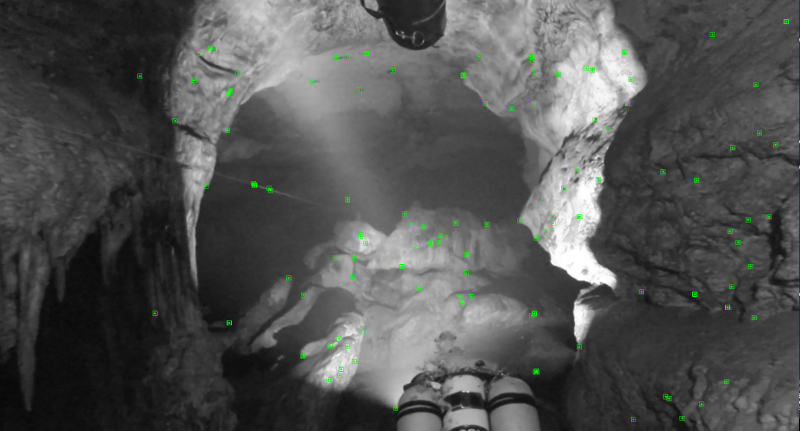
\includegraphics[width=0.9\textwidth]{./figures/OrbFeaturesS}}
 	\caption{ORB features tracked by ORB\hyp SLAM 2.}\vspace{-0.2in}
 	\label{fig:OrbFeatures}
\end{figure}

Brute force application of VO algorithms~\cite{da2009visual,Corke} is quite challenging in the underwater cave domain, due to the lighting variations and the sharp contrasts existing in the image, as discussed earlier. However, by thresholding the image, the areas of adequate illumination in the left and right camera feed can be used to apply one of the latest VO algorithms, ORB\hyp SLAM 2, a variant of ORB\hyp SLAM~\cite{ORB1,murTRO2015} for stereo vision. Figure \ref{fig:OrbFeatures} presents tracked features in the areas with higher illumination. It is worth noting that during some segments of the video the third diver swimming below the camera exhaled sending a cloud of bubbles in the field of view, however, the VO algorithm was robust enough to handle these dynamic features. This event highlighted one of the challenges of underwater vision. 

\begin{figure*}[ht]
	\begin{center}
		\leavevmode
		\begin{tabular}{cc}
			\subfloat[]{\fbox{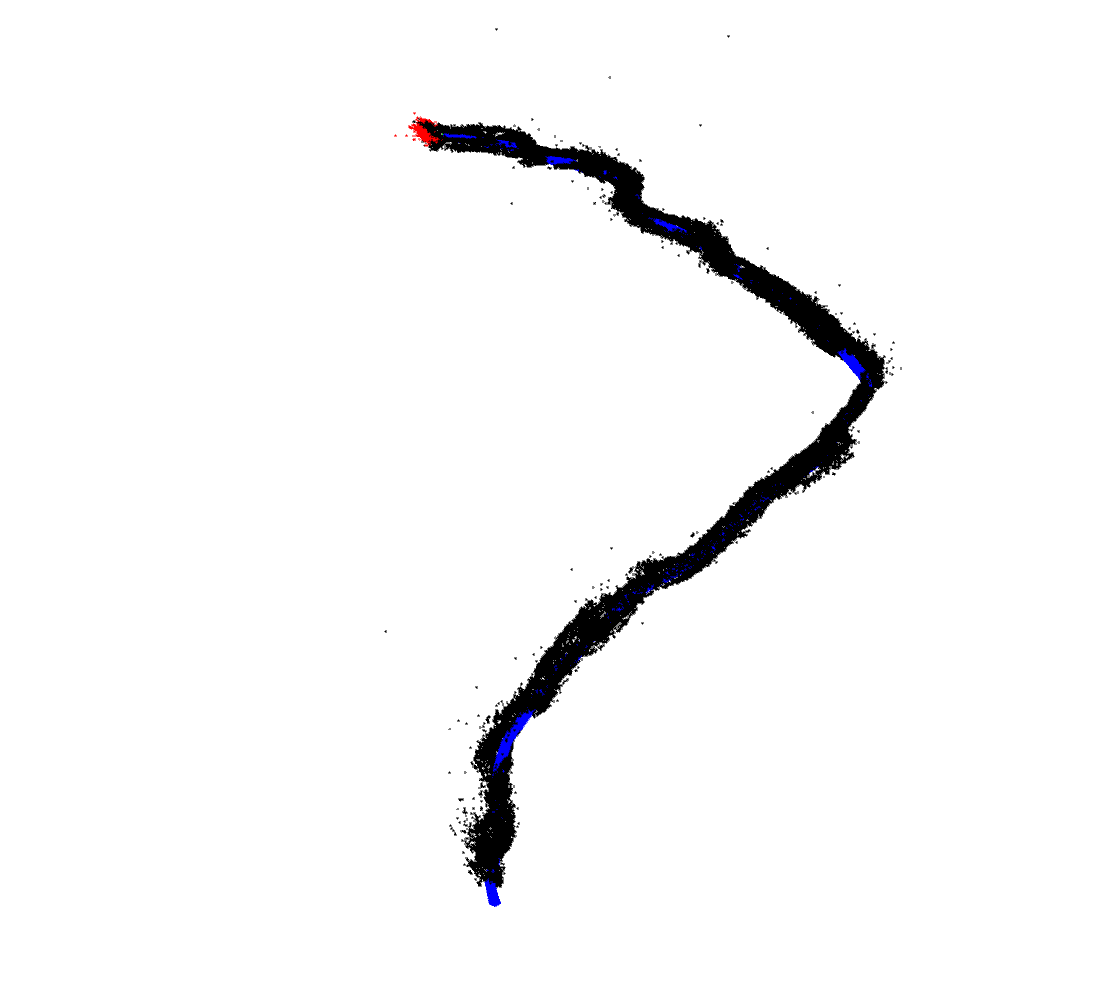
\includegraphics[height=0.41\textheight, clip=true, trim=3.0in 0.0in 2.0in 0.0in]{./figures/8_min_ORBSLAM}\label{fig:orb1}}}&
			\subfloat[]{\fbox{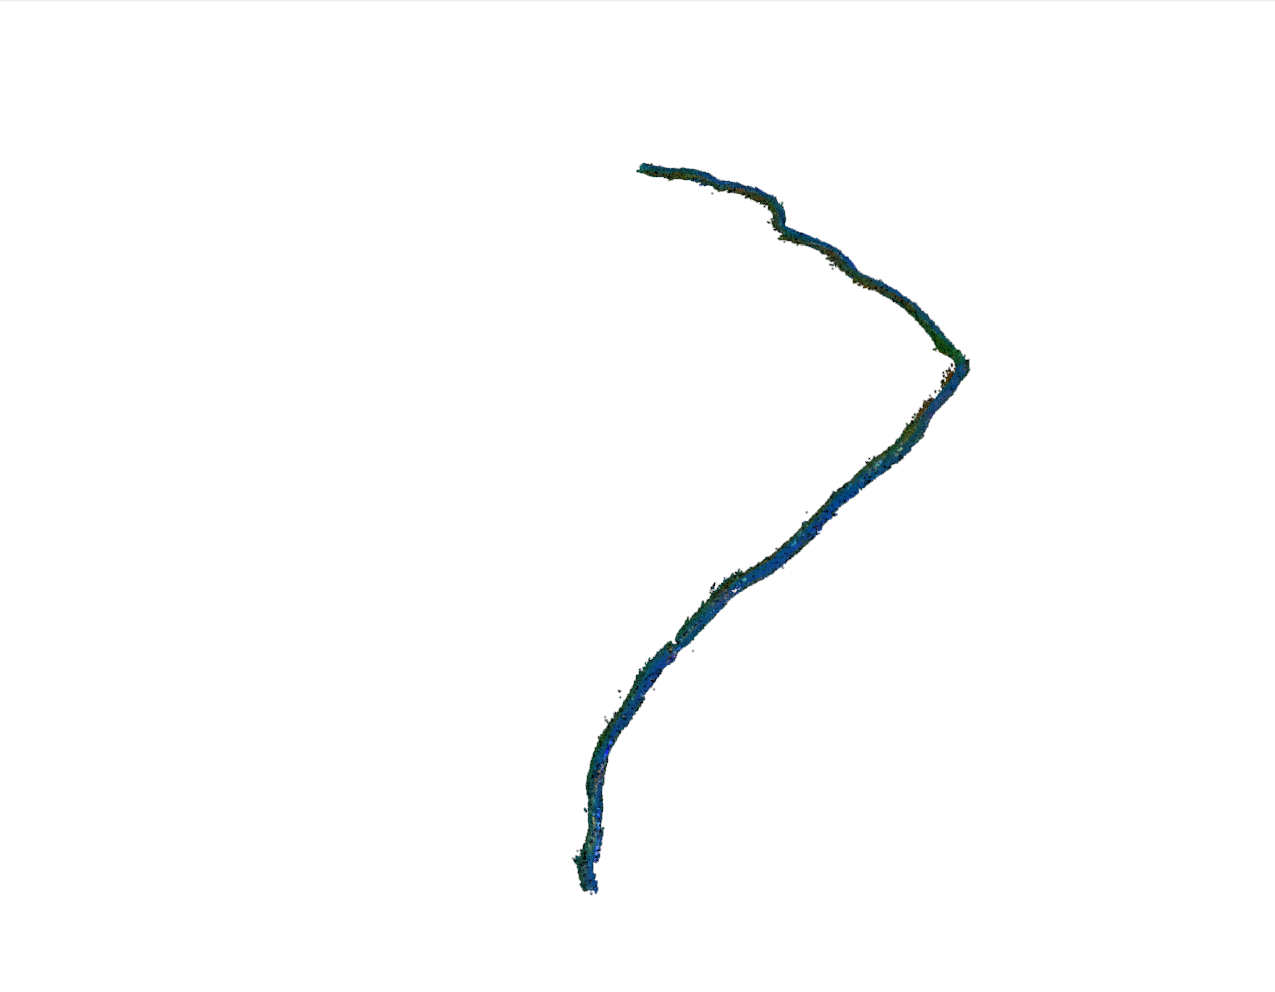
\includegraphics[height=0.41\textheight, clip=true, trim=5.0in 0.0in 2.50in 0.0in]{./figures/8_min_Our_Method}\label{fig:orb2}}}
		\end{tabular}
		\caption{\ref{fig:orb1} The trajectory calculated by ORB\hyp SLAM 2 of a 7 min 28 sec traversal and the 3\hyp D points estimated from ORB features. \ref{fig:orb2} The wireframe reconstructed from the proposed stereo algorithm. Please note, the reduced number of outliers compared to  \ref{fig:orb1}.}
		\label{fig:orb}
	\end{center}
\end{figure*}

Figure \ref{fig:orb} presents the trajectory of the stereo camera and the 3\hyp D position of stable features as extracted from ORB\hyp SLAM 2 from a trajectory of seven minutes, twenty eight seconds. While there was no ground truth, observing the video one gets a qualitative verification for the estimated trajectory. The estimated trajectory is then used as an input to produce a volumetric map by transforming the boundaries calculated above through space using the estimated pose of the stereo camera at each instant. It is clear that the contour based reconstruction; see Fig. \ref{fig:orb1}, has eliminated several outliers which were present in the ORB-SLAM reconstruction; see Fig. \ref{fig:orb2}. The next section presents results from an actual cave.